\documentclass[fleqn,10pt]{wlscirep}
\usepackage[utf8]{inputenc}
\usepackage[T1]{fontenc}
\usepackage{lineno}

\linenumbers

\title{Microelectrode electrophysiology: Extending the Brain Imaging Data Structure to intracellular and extracellular recordings in animal models}

% Following author list patterns from Pernet2019 (EEG-BIDS: 24 authors), Holdgraf2019 (iEEG-BIDS: 44 authors)
\author[1,*]{First Author}
% Add 20-40 authors representing diverse stakeholders as per successful extensions

\begin{abstract}
% This is a manuscript template for Data Descriptor submissions to \emph{Scientific Data} (\href{http://www.nature.com/scientificdata}{http://www.nature.com/scientificdata}). The abstract must be no longer than 170 words, and should succinctly describe the study, the assay(s) performed, the resulting data, and the reuse potential, but should not make any claims regarding new scientific findings. No references are allowed in this section.

% Following Scientific Data format - 170 words max, no references
% Pattern from Pernet2019, Niso2018, Holdgraf2019
The Brain Imaging Data Structure (BIDS) has facilitated data sharing and tool development in human neuroimaging.
We present an extension for microelectrode electrophysiology recordings in animal models, addressing the unique requirements of intracellular and extracellular recordings.
This extension introduces two new data types: 'icephys' for intracellular and 'ecephys' for extracellular recordings, supporting diverse recording modalities from patch-clamp to high-density silicon probes.
Building on existing BIDS principles and prior electrophysiology extensions, we specify metadata for probes, electrodes, and channels, with particular attention to metadata required for spike sorting analysis.
The extension adopts NWB (Neurodata Without Borders) and NIX (Neuroscience Information Exchange) as data formats, ensuring comprehensive metadata capture while maintaining compatibility with existing analysis ecosystems.
We provide example datasets covering common use cases and demonstrate integration with established tools including [Which tools?].
This standardization enables reproducible analysis pipelines, facilitates data sharing through repositories like DANDI, G-Node and EBRAINS, and bridges scales from cellular to systems neuroscience.
\end{abstract}

\begin{document}

\flushbottom
\maketitle
%  Click the title above to edit the author information and abstract

\thispagestyle{empty}

% \noindent Please note: Abbreviations should be introduced at the first mention in the main text – no abbreviations lists or tables should be included. Structure of the main text is provided below.

\section*{Background \& Summary}

% (700 words maximum) An overview of the study design, the assay(s) performed, and the created data, including any background information needed to put this study in the context of previous work and the literature. The section should also briefly outline the broader goals that motivated the creation of this dataset and the potential reuse value. We also encourage authors to include a figure that provides a schematic overview of the study and assay(s) design. The Background \& Summary should not include subheadings. This section and the other main body sections of the manuscript should include citations to the literature as needed.

% 700 words max, following structure from Gorgolewski2016, Pernet2019, Holdgraf2019

% Paragraph 1: Field context and technological advances
% Following Pernet2019 opening
Microelectrode electrophysiology encompasses techniques for recording electrical activity from individual neurons to local field potentials, providing crucial insights into neural computation.
Recent technological advances, including high-density silicon probes and standardized probe designs through the Neuropixels project, have dramatically increased data acquisition rates and experimental complexity.
% Add statistics on data growth, number of labs using these techniques

% Paragraph 2: Current standardization landscape and fragmentation
% Following pattern from Holdgraf2019, Niso2018
While comprehensive data formats exist for neurophysiology (NWB; NIX),
the field lacks standardized organization principles for datasets, metadata specifications, and directory structures.
This fragmentation impedes data sharing, with surveys indicating [ADD SURVEY DATA] of researchers struggling to share or reuse electrophysiology data due to inconsistent formats and missing metadata.
% Reference Neo, existing tools showing fragmentation

% Paragraph 3: BIDS success and extension rationale
% Following Gorgolewski2016, Poldrack2024
BIDS has successfully standardized human neuroimaging data organization [cite],
with over 850 datasets on OpenNeuro [cite] and adoption by major repositories.
Prior BIDS extensions for human electrophysiology (EEG [cite], MEG [cite], iEEG [cite])
established patterns for organizing time-series neural data, while the Microscopy extension [cite]
introduced critical metadata fields for animal data.

% Paragraph 4: Unique challenges for microelectrophysiology
% New content specific to BEP032
Microelectrode recordings present unique challenges:
(1) electrode scales spanning orders of magnitude (sub-micron tips to millimeter arrays),
(2) diverse probe geometries requiring specialized coordinate systems,
(3) spike sorting as an essential preprocessing step requires specific metadata,

% Paragraph 5: Extension overview and contributions
Here we present BEP032, extending BIDS to microelectrode electrophysiology, with a focus on animal models.
This extension: [summarize key contributions]
% List main contributions following Holdgraf2019 pattern

% Include Figure 1: Schematic overview (following Pernet2019 Fig 1, Bourget2022 Fig 1)
% Show directory structure, data flow, and relationship to other modalities

\section*{Methods}

% The Methods should include detailed text describing any steps or procedures used in producing the data, including full descriptions of the experimental design, data acquisition assays, and any computational processing (e.g. normalization, image feature extraction). See the detailed section in our submission guidelines for advice on writing a transparent and reproducible methods section. Related methods should be grouped under corresponding subheadings where possible, and methods should be described in enough detail to allow other researchers to interpret and repeat, if required, the full study. Specific data outputs should be explicitly referenced via data citation (see Data Records and Citing Data, below).

% Authors should cite previous descriptions of the methods under use, but ideally the method descriptions should be complete enough for others to understand and reproduce the methods and processing steps without referring to associated publications. There is no limit to the length of the Methods section. Subheadings should not be numbered.

% \subsection*{Subsection}

% Example text under a subsection. Bulleted lists may be used where appropriate, e.g.

% \begin{itemize}
% \item First item
% \item Second item
% \end{itemize}

% \subsubsection*{Third-level section}

\subsection*{Community Development Process}
% Following detailed process documentation from Pernet2019 Section "BIDS-EEG: the process"
% Timeline following ASL-BIDS pattern

The development of BEP032 began in [DATE] through the INCF Working Group on Standardized Data Structures.
% Document meetings, consultations, public comment periods
% Include stakeholder groups table as in Holdgraf2019

\subsection*{Scope and Design Principles}
% Following Niso2018 "Scope" section

\subsubsection*{Inclusion Criteria}
% Define what's included: patch clamp, sharp electrode, extracellular, etc.

\subsubsection*{Design Decisions}
% Following MEG-BIDS choice to not require format conversion
% Justify NIX/NWB requirement vs allowing native formats
% Discuss division between icephys and ecephys

The division between intracellular (icephys) and extracellular (ecephys) electrophysiology is based on the recording techniques and the resulting data characteristics. Icephys typically involves high-resolution recordings from individual neurons, requiring detailed metadata about the cell type, location, and experimental conditions. In contrast, ecephys captures broader population activity, necessitating metadata that describes the electrode array configuration, spatial sampling, and signal processing methods.

\subsection*{Directory Structure and File Organization}
% Following pattern from all electrophysiology papers

\subsubsection*{Data Type Specification}
% Explain icephys vs ecephys separation
% Reference Table showing directory structure

\subsubsection*{Required and Optional Files}
% Table following Pernet2019 Table 1, Holdgraf2019 Table 2

\subsection*{Metadata Specifications}

\subsubsection*{Inheritance Principle}
% Following Gorgolewski2016 explanation

\subsubsection*{Required Metadata Fields}
% Table with field, description, and justification
% Pattern from Pernet2019 Table 3, Niso2018 Table 3

\subsubsection*{Animal-Specific Metadata}
% Building on Bourget2022
% Species, strain, age handling

\subsection*{Probe, Electrode, and Channel Specifications}
% Core technical content following iEEG-BIDS electrode handling

\subsubsection*{Probes TSV Specification}
% New for microelectrophysiology
% Table with required/optional columns

\subsubsection*{Electrodes TSV Specification}
% Adapt from Holdgraf2019
% Handle 3D coordinates, impedance

\subsubsection*{Channels TSV Specification}
% Extend Pernet2019 channel types
% Added channel types for microelectrophysiology

\subsection*{Coordinate Systems}
% Following Holdgraf2019 Section 2.4

\subsubsection*{Stereotaxic Coordinates}
% Bregma/lambda reference for rodents

\subsubsection*{Atlas-Based Coordinates}
% Allen CCF, Paxinos references

\subsubsection*{Probe-Relative Coordinates}

\subsection*{Spike Sorting and Derivatives}
% New section critical for microelectrophysiology
% Justifying sufficient metadata for spike sorting

\subsection*{Integration with Existing Tools}
% Following Pernet2019 Section 4
% nuroconv - to NWB/NIX

\subsubsection*{Conversion Tools}
% nwb2bids

\subsubsection*{Analysis Pipelines}
% Compatibility demonstration

% Topical subheadings are allowed.

\section*{Data Records}

% The Data Records section should be used to explain each data record associated with this work, including the repository where this information is stored, and to provide an overview of the data files and their formats. Each external data record should be cited numerically in the text of this section, for example \cite{Hao:gidmaps:2014}, and included in the main reference list as described below. A data citation should also be placed in the subsection of the Methods containing the data-collection or analytical procedure(s) used to derive the corresponding record. Providing a direct link to the dataset may also be helpful to readers (\hyperlink{https://doi.org/10.6084/m9.figshare.853801}{https://doi.org/10.6084/m9.figshare.853801}).

% Tables should be used to support the data records, and should clearly indicate the samples and subjects (study inputs), their provenance, and the experimental manipulations performed on each (please see 'Tables' below). They should also specify the data output resulting from each data-collection or analytical step, should these form part of the archived record.

% Following Bourget2022, Holdgraf2019 pattern

Example datasets demonstrating the specification are available at [REPOSITORY].
Table~\ref{tab:datasets} summarizes the datasets, recording techniques, and use cases.

% Table: Example datasets
% Columns: Dataset name, Species, Recording type, Probe type, Duration, Size, DOI

\subsection*{Dataset 1: One icephys dataset}
% Brief description, link to repository

\subsection*{Dataset 2: One chronic ecephys dataset}
% Brief description, link to repository

\subsection*{Dataset 3: One acute ecephys experiment}
% Brief description, link to repository

\subsection*{Dataset 4: Neuropixels Multi-Region Recording}
% Brief description, link to repository

\section*{Technical Validation}

% This section presents any experiments or analyses that are needed to support the technical quality of the dataset. This section may be supported by figures and tables, as needed. This is a required section; authors must present information justifying the reliability of their data.

% Following Pernet2019, Niso2018 validation approaches

\subsection*{Validator Compliance}
% BIDS validator extension testing

\subsection*{Round-Trip Conversion}
% Demonstrate data integrity through conversion

\subsection*{Cross-Tool Compatibility}
% Test with multiple analysis pipelines

\subsection*{File Size and Performance}
% Address scalability for large datasets


\section*{Usage Notes}

% The Usage Notes should contain brief instructions to assist other researchers with reuse of the data. This may include discussion of software packages that are suitable for analysing the assay data files, suggested downstream processing steps (e.g. normalization, etc.), or tips for integrating or comparing the data records with other datasets. Authors are encouraged to provide code, programs or data-processing workflows if they may help others understand or use the data. Please see our code availability policy for advice on supplying custom code alongside Data Descriptor manuscripts.

% For studies involving privacy or safety controls on public access to the data, this section should describe in detail these controls, including how authors can apply to access the data, what criteria will be used to determine who may access the data, and any limitations on data use.

% Following all papers' patterns

\subsection*{Converting Existing Data}
% Step-by-step guide
% neuroconv, MNE-BIDS create structure?? any other tool?

\subsection*{Recommended Workflows}
% Best practices for organization

\subsection*{Integration with Other Modalities}
% Combining with imaging, behavior

\subsection*{Repository Submission}
% DANDI, GIN guidance

\section*{Code availability}

% For all studies using custom code in the generation or processing of datasets, a statement must be included under the heading "Code availability", indicating whether and how the code can be accessed, including any restrictions to access. This section should also include information on the versions of any software used, if relevant, and any specific variables or parameters used to generate, test, or process the current dataset.

% Following standard format

BEP032tools [VERSION] provides validation and conversion utilities: [GITHUB LINK]
Example conversion scripts are available at: [GITHUB LINK]
The specification is maintained at: https://github.com/bids-standard/bids-specification

\bibliography{bep032}

% \noindent LaTeX formats citations and references automatically using the bibliography records in your .bib file, which you can edit via the project menu. Use the cite command for an inline citation, e.g. \cite{Kaufman2020, Figueredo:2009dg, Babichev2002, behringer2014manipulating}. For data citations of datasets uploaded to e.g. \emph{figshare}, please use the \verb|howpublished| option in the bib entry to specify the platform and the link, as in the \verb|Hao:gidmaps:2014| example in the sample bibliography file. For journal articles, DOIs should be included for works in press that do not yet have volume or page numbers. For other journal articles, DOIs should be included uniformly for all articles or not at all. We recommend that you encode all DOIs in your bibtex database as full URLs, e.g. https://doi.org/10.1007/s12110-009-9068-2.

\section*{Acknowledgements}
% Acknowledge working group, funders, community contributors

% Acknowledgements should be brief, and should not include thanks to anonymous referees and editors, or effusive comments. Grant or contribution numbers may be acknowledged.

\section*{Author Contributions}
% Following Holdgraf2019 detailed contributions

% Must include all authors, identified by initials, for example:
% A.A. conceived the experiment(s), A.A. and B.A. conducted the experiment(s), C.A. and D.A. analysed the results. All authors reviewed the manuscript.

\section*{Competing Interests}
The authors declare no competing interests.

% The corresponding author is responsible for providing a \href{https://www.nature.com/sdata/policies/editorial-and-publishing-policies#competing}{competing interests statement} on behalf of all authors of the paper. This statement must be included in the submitted article file.

\section*{Figures \& Tables}

% Figures, tables, and their legends, should be included at the end of the document. Figures and tables can be referenced in \LaTeX{} using the ref command, e.g. Figure \ref{fig:stream} and Table \ref{tab:example}.

% Authors are encouraged to provide one or more tables that provide basic information on the main 'inputs' to the study (e.g. samples, participants, or information sources) and the main data outputs of the study. Tables in the manuscript should generally not be used to present primary data (i.e. measurements). Tables containing primary data should be submitted to an appropriate data repository.

% Tables may be provided within the \LaTeX{} document or as separate files (tab-delimited text or Excel files). Legends, where needed, should be included here. Generally, a Data Descriptor should have fewer than ten Tables, but more may be allowed when needed. Tables may be of any size, but only Tables which fit onto a single printed page will be included in the PDF version of the article (up to a maximum of three).

% Due to typesetting constraints, tables that do not fit onto a single A4 page cannot be included in the PDF version of the article and will be made available in the online version only. Any such tables must be labelled in the text as 'Online-only' tables and numbered separately from the main table list e.g. 'Table 1, Table 2, Online-only Table 1' etc.

\begin{figure}[ht]
\centering
% Figure 1: Overview schematic
\caption{Overview of the BIDS microelectrode electrophysiology extension.
(a) Directory structure showing icephys and ecephys datatypes.
(b) Metadata inheritance hierarchy.
(c) Relationship between probes, electrodes, and channels.
(d) Integration with analysis tools and repositories.}
\label{fig:overview}
\end{figure}

% \begin{figure}[ht]
% \centering
% 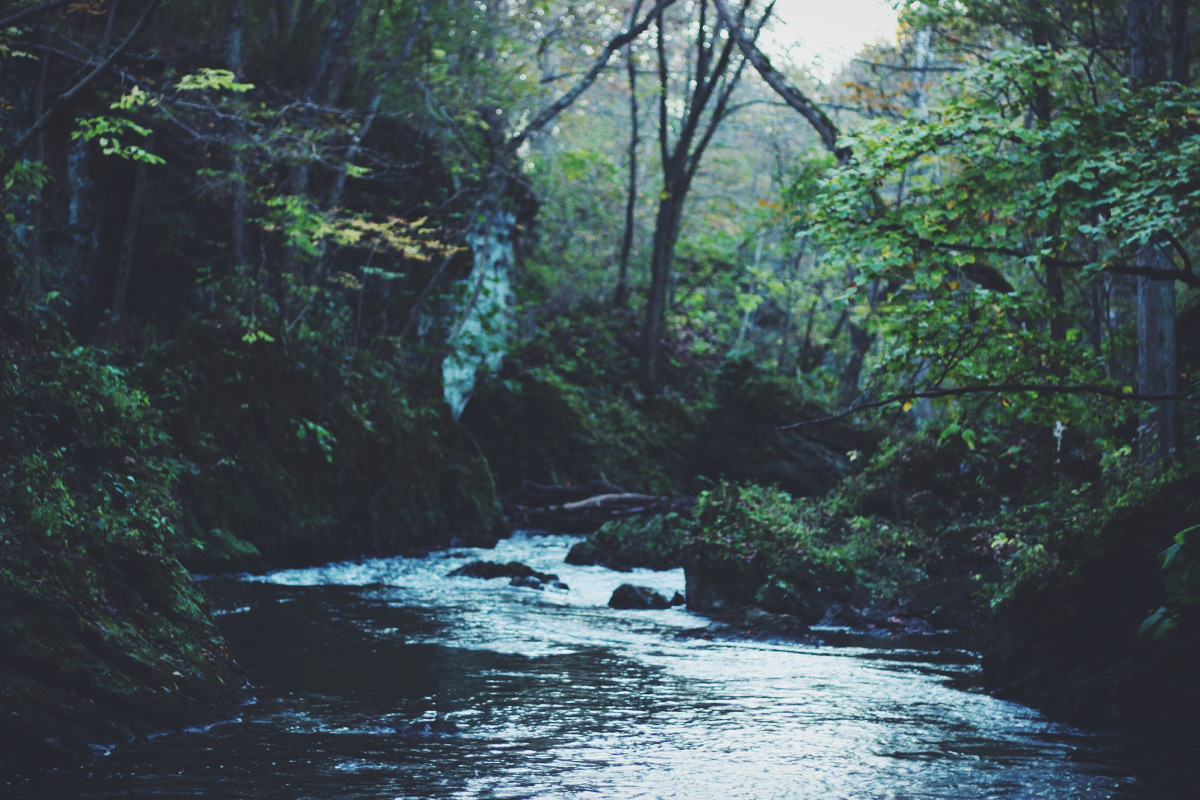
\includegraphics[width=\linewidth]{stream}
% \caption{Legend (350 words max). Example legend text.}
% \label{fig:stream}
% \end{figure}

\begin{table}[ht]
\centering
\caption{Required and optional files for microelectrode electrophysiology recordings}
% Following Pernet2019 Table 1 format
\label{tab:files}
\end{table}

\begin{table}[ht]
\centering
\caption{Required metadata fields and their descriptions}
% Following Niso2018 Table 3 format
\label{tab:metadata}
\end{table}

\begin{table}[ht]
\centering
\caption{Channel types for microelectrode recordings}
% Extending Pernet2019 Table 2
\label{tab:channels}
\end{table}

\begin{table}[ht]
\centering
\caption{Example datasets demonstrating the specification}
\label{tab:datasets}
\end{table}

% Online-only tables if needed for comprehensive metadata listings

% \begin{table}[ht]
% \centering
% \begin{tabular}{|l|l|l|}
% \hline
% Condition & n & p \\
% \hline
% A & 5 & 0.1 \\
% \hline
% B & 10 & 0.01 \\
% \hline
% \end{tabular}
% \caption{\label{tab:example}Legend (350 words max). Example legend text.}
% \end{table}

\end{document}